\def \currentAuthor {Gabi Sorglos} %so kann jederzeit der Autor geändert werden -> wird in der Fusszeile angezeigt.

\chapter*{Einleitende Bemerkungen}

\chapter*{Notationen}
Beschreibung wie Code, Hinweise, Zitate etc. formatiert werden  

\chapter{Projektmanagement}

\section{Metainformationen}
\subsection{Team}
\subsection{Betreuer}
\subsection{Partner}
\subsection{Ansprechpartner}
\section{Vorerhebungen}
\subsection{Projektzieleplan}
Projektziele-Hierarchie - SMART
\newpage
\subsection{Projektumfeld}
\begin{itemize}
	\item Identifikation der Stakeholder
	\item Charakterisierung der Stakeholder
	\item Maßnahmen
	\item Grafische Darstellung des Umfeldes
\end{itemize}
\subsection{Risikoanalyse}
\subsubsection{Risikoidentifikation}
Folgende Risiken können während der Projektdurchführung erwartet werden:
\begin{itemize}
	\item[\textbf{R1}] Projektmitglied steig aus dem Projekt aus.
	\item[\textbf{R2}] Projektpartner stellt seine Kooperation ein.
	\item[\textbf{R3}] Projektpartner ändert seine Anforderungen.
	\item[\textbf{R4}] Termine können nicht eingehalten werden.
	\item[\textbf{R5}] Anforderungen werden nicht erreicht.			
\end{itemize}

\subsubsection{Bewertung und Behandlung}
Die aufgelisteten Risiken werden nach Auswirkung und Eintrittswahrscheinlichkeit bewertet.
Je höher die Zahl in der Tabelle, desto höher ist die Auswirkung bzw. Einwirkung.
\begin{table}[h]
	\begin{tabular}{l|c|c}
		\textbf{Risiko}                           & \multicolumn{1}{l|}{\textbf{Wahrscheinlichkeit}} & \multicolumn{1}{l}{\textbf{Auswirkung}} \\ \hline
		\textbf{R1} Ausstieg Projektmitglied                  & 3                                                & 10                                      \\
		\textbf{R2} Projektpartner stellt Kooperation ein     & 2                                                & 10                                      \\
		\textbf{R3} Projektpartner ändert seine Anforderungen & 4                                                & 7                                       \\
		\textbf{R4} Termine können nicht eingehalten werden   & 3                                                & 6                                       \\
		\textbf{R5} Anforderungen werden nicht erreicht       & 2                                                & 8                                      
	\end{tabular}
	\caption{Analyse Einwirkung \& Auswirkung}
	\label{Abb_Einwirkung_Auswirkung}
\end{table}

\subsubsection{Risikomatrix}
\begin{figure}[h]
	\centering
	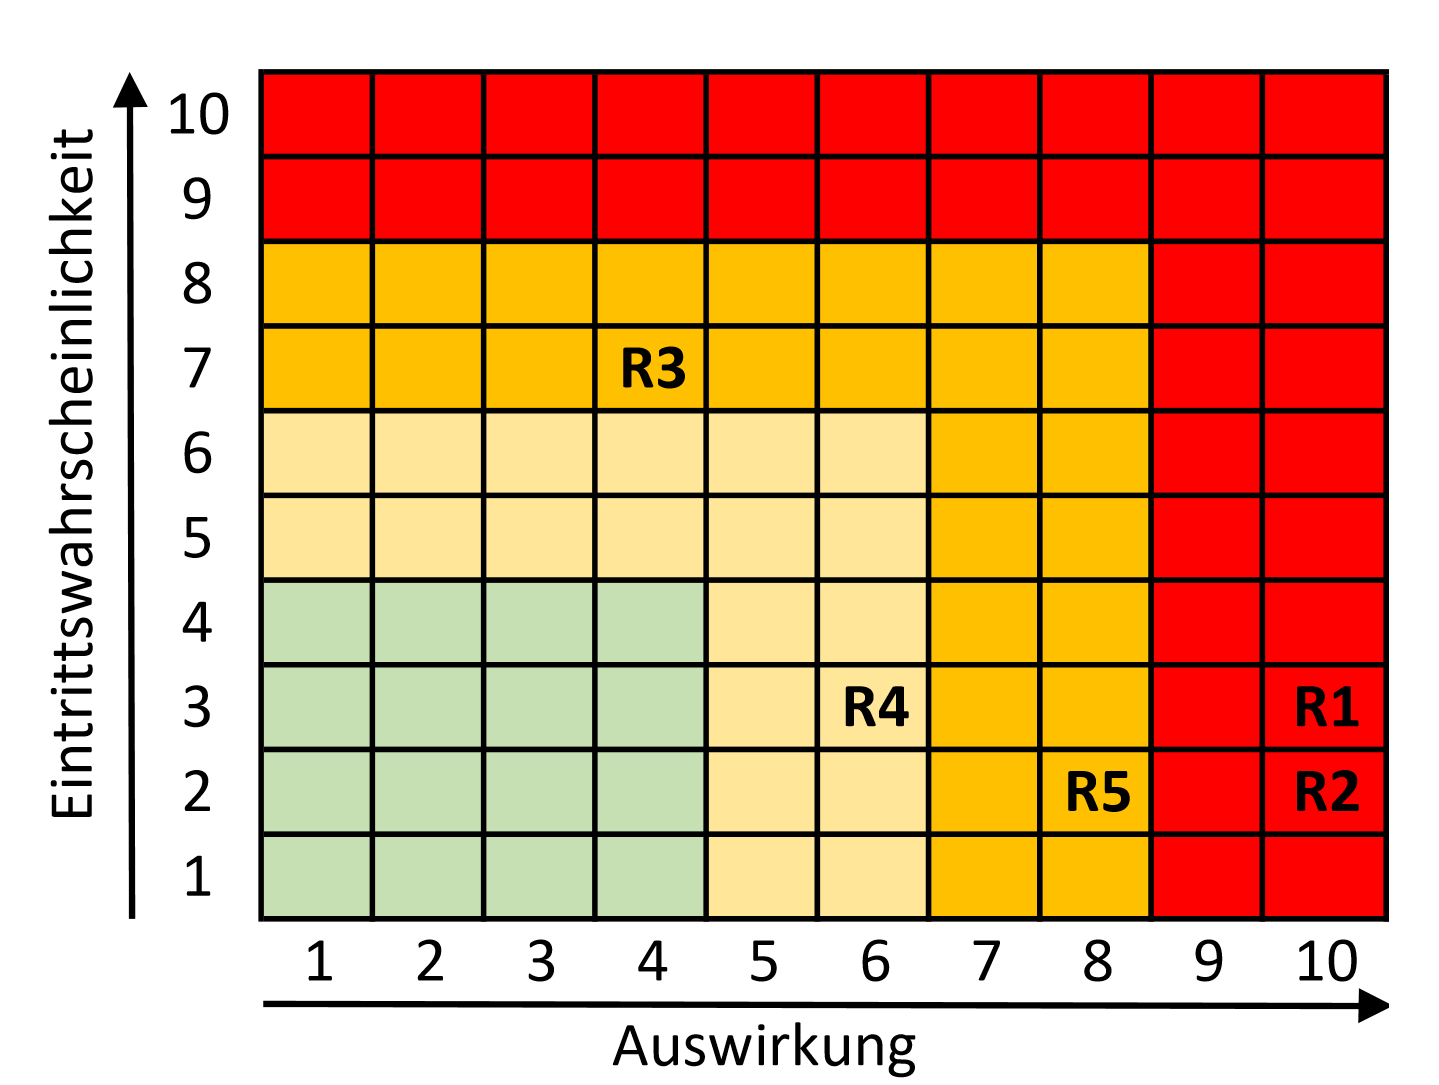
\includegraphics[scale=0.6]{figures/matrix.png}
	\caption{Risikomatrix}
	\label{Abb_Risikomatrix}
\end{figure}

\section{Pflichtenheft}
\subsection{Zielbestimmung}
\begin{itemize}
	\item Projektbeschreibung
	\item IST-Zustand
	\item SOLL-Zustand
	\item NICHT-Ziele (Abgrenzungskriterien)
\end{itemize}
\subsection{Produkteinsatz und Umgebung}
\begin{itemize}
	\item Anwendungsgebiet
	\item Zielgruppen
	\item Betriebsbedingungen
	\item Hard-/Softwareumgebung
\end{itemize}
\subsection{Funktionalitäten}
\begin{itemize}
	\item MUSS-Anforderungen
	\begin{itemize}
		\item Funktional
		\item Nicht-funktional
	\end{itemize}
	\item KANN-Anforderungen
	\begin{itemize}
		\item Funktional
		\item Nicht-funktional
	\end{itemize}
\end{itemize}
\subsection{Testszenarien und Testfälle}
\begin{itemize}
	\item Beschreibung der Testmethodik
	\item Testfall 1
	\item Testfall 2
	\item \ldots
\end{itemize}
\subsection{Liefervereinbarung}
\begin{itemize}
	\item Lieferumfang
	\item Modus
	\item Verteilung(Deployment)
\end{itemize}
\section{Planung}
\subsection{Projektstrukturplan}
\subsection{Meilensteine}
\subsection{Gant-Chart}
\subsection{Abnahmekriterien}
\subsection{Pläne zur Evaluierung}
\subsection{Ergänzungen und zu klärende Punkte}

\chapter{Vorstellung des Produktes}
Vorstellung des fertigen Produktes anhand von Screenshots, Bildern, Erklärungen.

\chapter{Eingesetzte Technologien}
\begin{itemize}
	\item Kurzbeschreibung aller Technologien, die verwendet wurden.
	\item Technologien die aus dem Unterricht bekannt sind, nur nennen und deren  Einsatzzweck im Projekt beschreiben, nicht die Technologien selbst.
	\item Technologien die aus dem Unterricht nicht bekannt sind, im Detail beschreiben incl. deren Einsatz im Projekt
	\item Fokus aus eingesetzten Frameworks
\end{itemize}

\chapter{Problemanalyse}
\section{USE-Case-Analyse}
\begin{itemize}
	\item UseCases auf Basis von Benutzerzielen identifizieren: 
	\begin{itemize}
		\item Benutzer eines Systems identifizieren
		\item Benutzerziele identifizieren (Interviews)
		\item Use-Case-Liste pro Benutzer definieren
	\end{itemize}
	\item UseCases auf Basis von Ereignissen identifizieren: 
	\begin{itemize}
		\item Externes Event triggert einen Prozess
		\item zeitliches Event triggert einen Prozess (Zeitpunkt wird erreicht) 
		\item State-Event (Zustandsänderung im System triggert einen Prozess)
	\end{itemize}
	\item Werkzeuge:
	\begin{itemize}
		\item USE-Case-Beschreibungen (textuell, tabellarisch)
		\item USE-Case-Diagramm
		\item Aktivitätsdiagramm für den Use-Case (Interaktion zwischen Akteur und System abbilden)
		\item System-Sequenzdiagramm (Spezialfall eines Sequenzdiagramms: Nur 1 Akteur und 1 Objekt, das Objekt ist das komplette System, es geht um die Input/Output Requirements, die abzubilden sind)
	\end{itemize}
\end{itemize}

\section{Domain-Class-Modelling}
\begin{itemize}
	\item "Dinge" (Rollen, Einheiten, Geräte, Events etc.) identifizieren, um die es im Projekt geht
	\item ER-Modellierung oder Klassendiagramme
	\item Zustandsdiagramme (zur Darstellung des Lebenszyklus von Domain-Klassen darstellen)
\end{itemize}

\section{User-Interface-Design}
\begin{itemize}
	\item Mockups
	\item Wireframes
\end{itemize}


\chapter{Systementwurf}

\section{Architektur}
Darstellung und Beschreibung der Systemarchitektur (z.B. Komponentendiagramme). 
Beispiele für Architekturen:

\begin{itemize}
	\item MVC
	\item Schichten
	\item Pipes
	\item Request Broker
	\item Service-Oriented
\end{itemize}

\section{Benutzerschnittstellen} 
Kompletter Entwurf aller Benutzerschnittstellen

\section{Datenbankentwurf}
Komplettes ER-Diagramm incl. Beschreibungen zu jeder einzelnen Tabelle und jeder Beziehung.

\section{Klassenentwurf}
Design jedes einzelnen USE-Cases

\begin{itemize}
	\item Design-Klassendiagramme vom Domain-Klassendiagramm ableiten (incl. detaillierter Darstellung und Verwendung von Vererbungshierarchichen, abstrakten Klassen, Interfaces)
	\item Sequenzdiagramme vom System-Sequenz-Diagramm ableiten
	\item 	Detaillierte Zustandsdiagramme für wichtige Klassen
\end{itemize}

Verwendung von CRC-Cards (Class, Responsibilities, Collaboration) für die Klassen
\begin{itemize}
	\item um Verantwortlichkeiten und Zusammenarbeit zwischen Klassen zu definieren und
	\item um auf den Entwurf der Geschäftslogik zu fokussieren
\end{itemize}

Design-Klassen für jeden einzelnen USE-Case können sein:
\begin{itemize}
	\item UI-Klassen
	\item Data-Access-Klassen
	\item Entity-Klassen (Domain-Klassen)
	\item Controller-Klassen
	\item Business-Logik-Klassen
	\item View-Klassen
\end{itemize}

Optimierung des Entwurfs (Modularisierung, Erweiterbarkeit, Lesbarkeit):
\begin{itemize}
	\item Kopplung optimieren
	\item 	Kohäsion optimieren
	\item 	SOLID
	\item 	Entwurfsmuster einsetzen
\end{itemize}

\section{Sicherheit des Systems}
Beschreibung aller sicherheitsrelevanten Designentscheidungen;

\chapter{Implementierung}
Detaillierte Beschreibung der Implementierung aller Teilkomponenten der Software entlang der zentralsten Use-Cases:

\begin{itemize}
	\item GUI-Implementierung
	\item Controllerlogik
	\item Geschäftslogik
	\item Datenbankzugriffe
\end{itemize}

Detaillierte Beschreibung der Teststrategie (Testdriven Development):

\begin{itemize}
	\item UNIT-Tests (Funktional)
	\item Integrationstests
\end{itemize}

Zu Codesequenzen:
\begin{itemize}
	\item kurze Codesequenzen direkt im Text (mit Zeilnnummern auf die man in der Beschreibung verweisen kann)
	\item lange Codesequenzen in den Anhang (mit Zeilennummer) und darauf verweisen (wie z.B. hier \cref{qj})
\end{itemize}

\chapter{Deployment}
\begin{itemize}
	\item Design der Ausführungsumgebung (Produktivenvironment)
	\item Umsetzung der Ausführungsumgebung
	\item Deployment
	\item DevOps-Thema
\end{itemize}

\chapter{Tests}

\section{Systemtests} 
Systemtests aller implementierten Funktionalitäten lt. Pflichtenheft
\begin{itemize}
	\item Beschreibung der Teststrategie
	\item Testfall 1
	\item Testfall 2
	\item Tesfall 3
	\item …
\end{itemize}

\section{Akzeptanztests}

\chapter{Projektevaluation}
siehe Projektmanagement-Unterricht

\chapter{Benutzerhandbuch} 
falls im Projekt gefordert

\chapter{Zusammenfassung}
\begin{itemize}
	\item Etwas längere Form des Abstracts
	\item Detaillierte Beschreibung des Outputs der Arbeit
\end{itemize}